\section{Prognostic Indicators}

\subsection{Survival Rates and Trends}

Survival rates in lung cancer are important indicators of disease burden, therapeutic success, and 
early detection effectiveness. These rates vary significantly depending on cancer type, stage at 
diagnosis, patient demographics, and treatment accessibility.

Non-small cell lung cancer (NSCLC), which comprises around 85\% of lung cancer cases, typically has 
a better prognosis than small cell lung cancer (SCLC), which is more aggressive and fast-growing. 
According to global cancer statistics, the 5-year survival rate for localized NSCLC is approximately 
64\%, but this rate drastically drops to 8\% for distant-stage disease \cite{cancerstats2023}.

In recent years, survival trends have improved slightly due to advances in early detection through 
low-dose CT screening, the development of targeted therapies, and immunotherapies. Studies have 
shown that overall mortality from lung cancer has declined in high-income countries, particularly in 
populations with reduced smoking rates and improved healthcare access \cite{siegeletc2022trends}.

\vspace{1em}
\begin{center}
    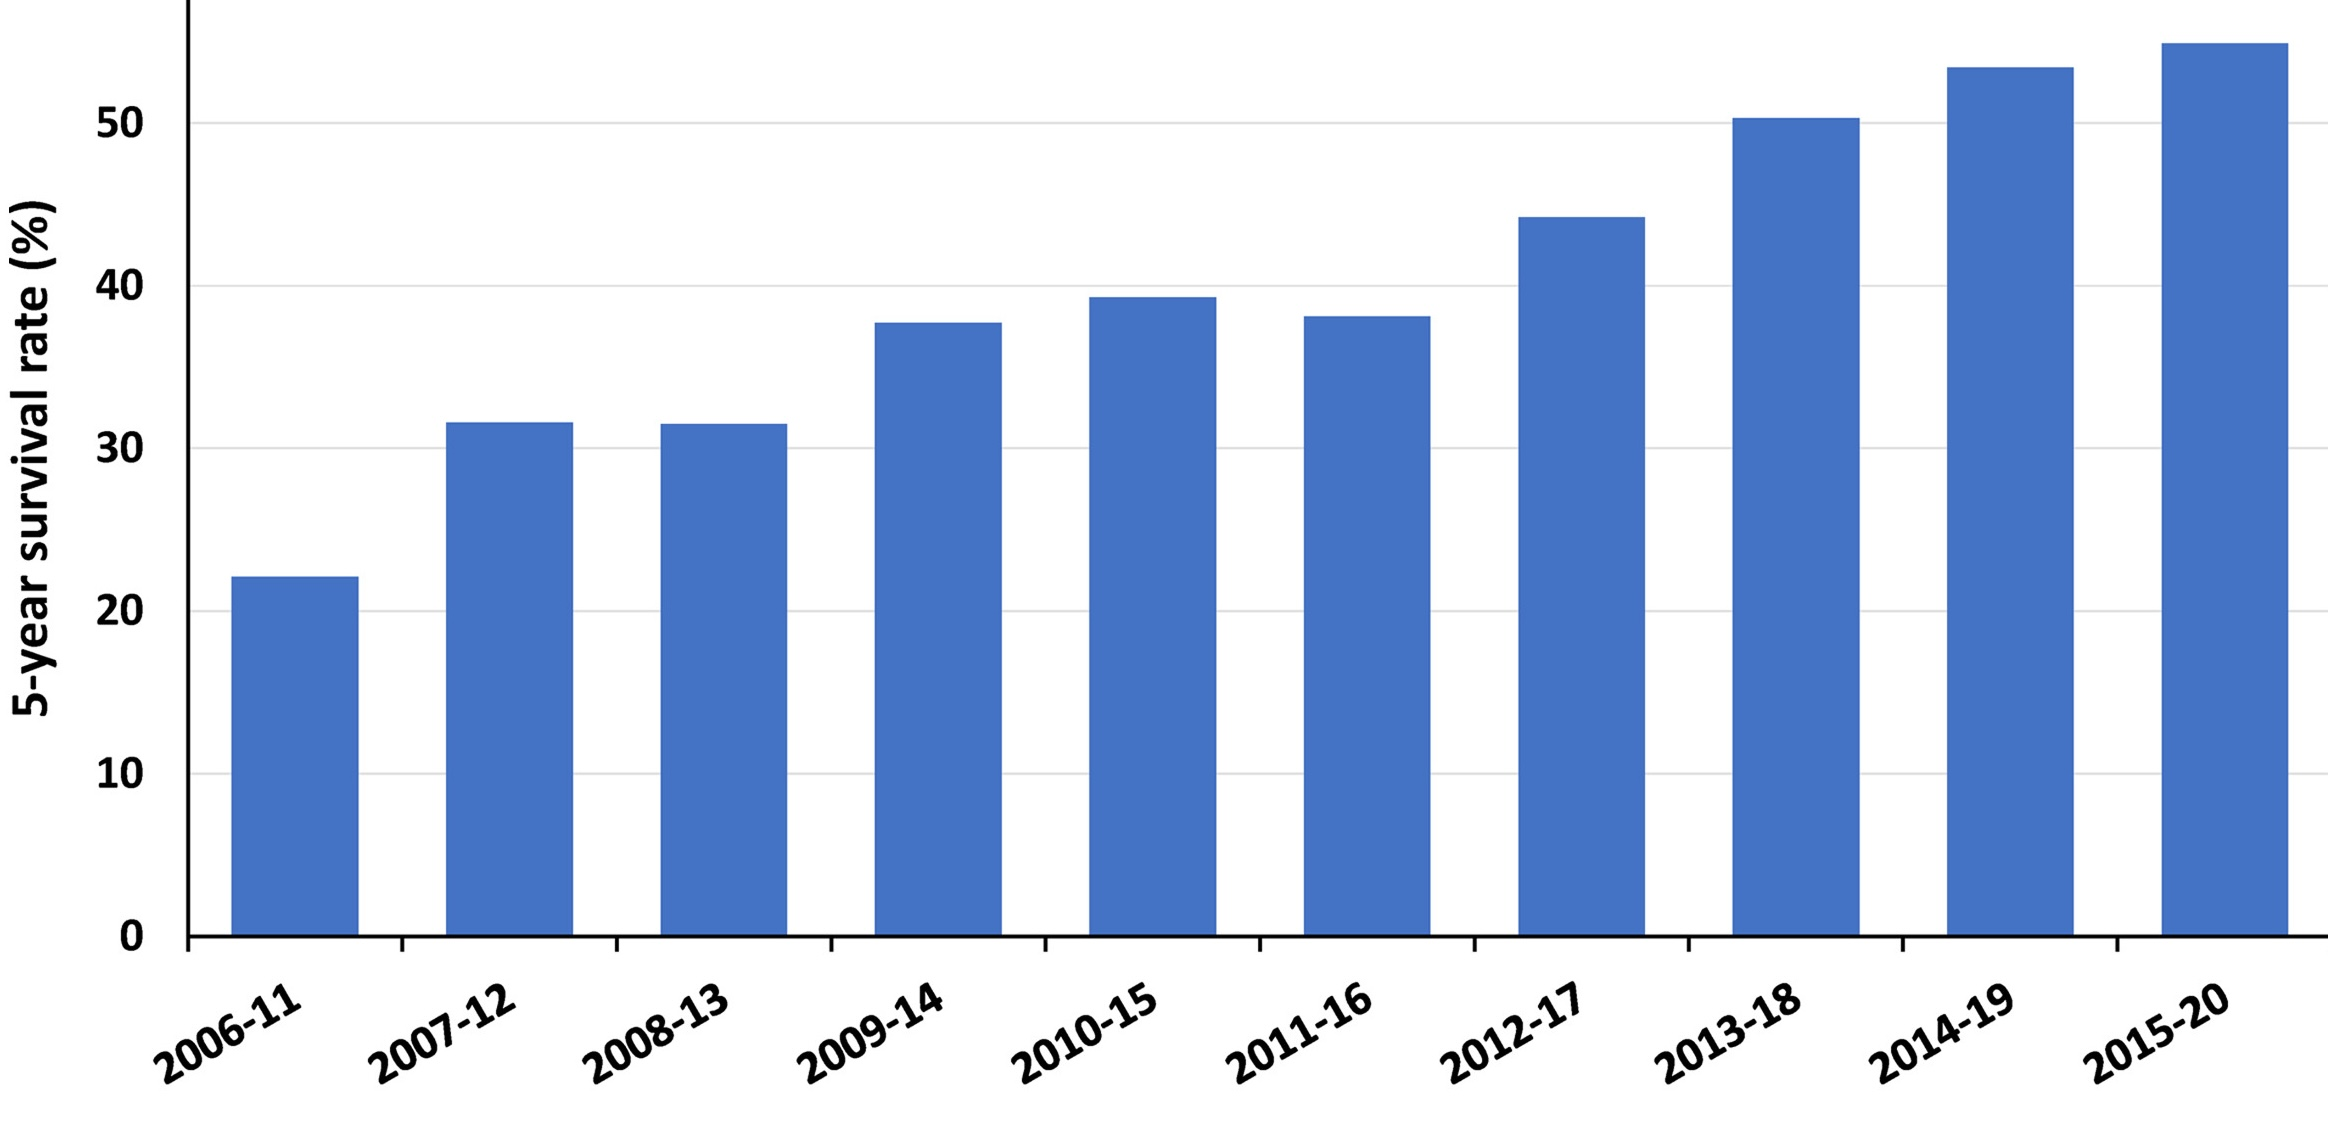
\includegraphics[width=1.00\textwidth]{../assets/05-prognosis/survival-rates.jpg}

    \small\textit{Five-year survival rates over years (all stages). \cite{osarogiagbon2023stage}}
\end{center}
\vspace{1em}

However, despite these improvements, lung cancer remains one of the leading causes of cancer-related 
deaths worldwide. The global 5-year survival rate for all lung cancers combined remains below 20\%, 
underlining the need for continued progress in early detection and treatment strategies 
\cite{bray2018global}.

\subsection{Determinants of Clinical Outcome}

Several clinical, biological, and lifestyle factors influence the prognosis of lung cancer patients. 
These determinants help clinicians estimate disease progression and tailor personalized treatment 
strategies.

\begin{itemize}
    \item \textbf{Stage at Diagnosis:} The single most important prognostic factor. Patients 
    diagnosed at early stages (I or II) typically have much better outcomes than those diagnosed at 
    advanced stages (III or IV). Early-stage lung cancer is often amenable to surgical resection or 
    curative radiotherapy, which significantly improves survival chances \cite{goldstaging}.
\end{itemize}

\vspace{1em}
\begin{center}
    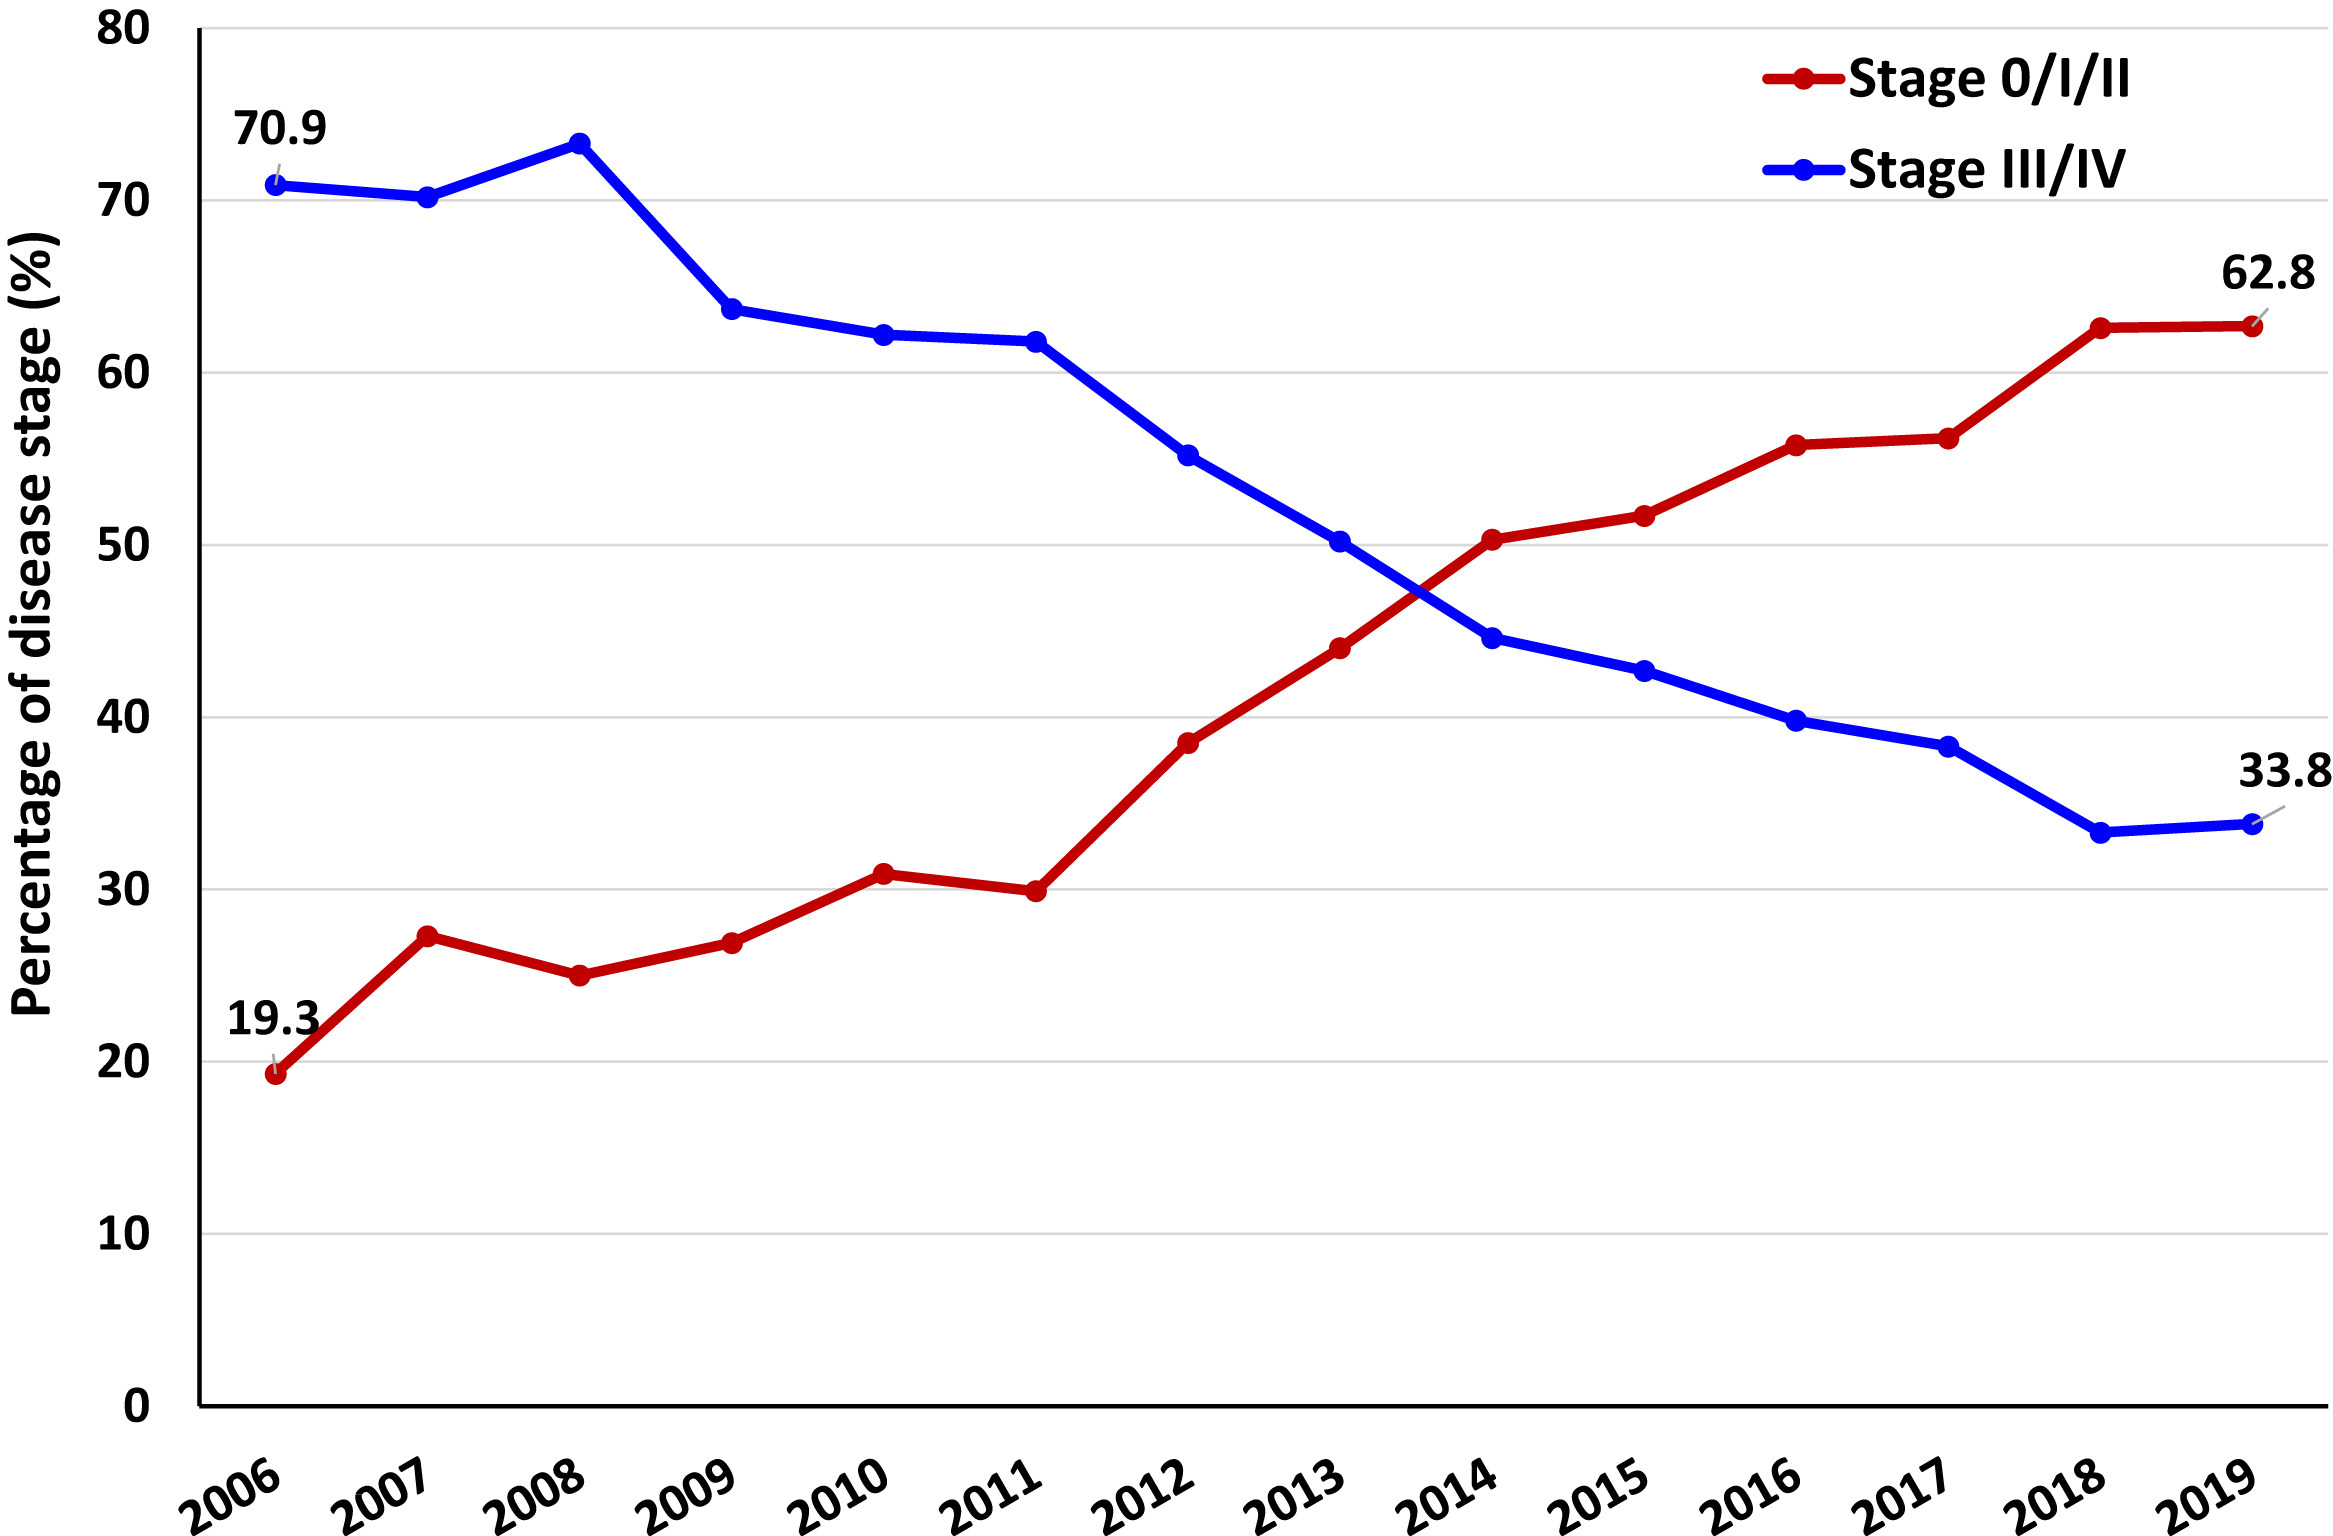
\includegraphics[width=1.00\textwidth]{../assets/05-prognosis/stage-survival-rates.jpg}

    \small\textit{Change in localized (stage 0/I/II) and advanced (stage III/IV) lung cancer from 
    2006 to 2019 in NTUH. NTUH, National Taiwan University Hospital. \cite{osarogiagbon2023stage}}
\end{center}
\vspace{1em}

\begin{itemize}
    \item \textbf{Histological Type:} The type of lung cancer, such as adenocarcinoma, squamous cell 
    carcinoma, or small cell carcinoma, impacts prognosis. For example, adenocarcinomas are 
    generally associated with better outcomes, while SCLC tends to have a more rapid progression and 
    worse prognosis \cite{travis2015classification}.
\end{itemize}

\vspace{1em}
\begin{center}
    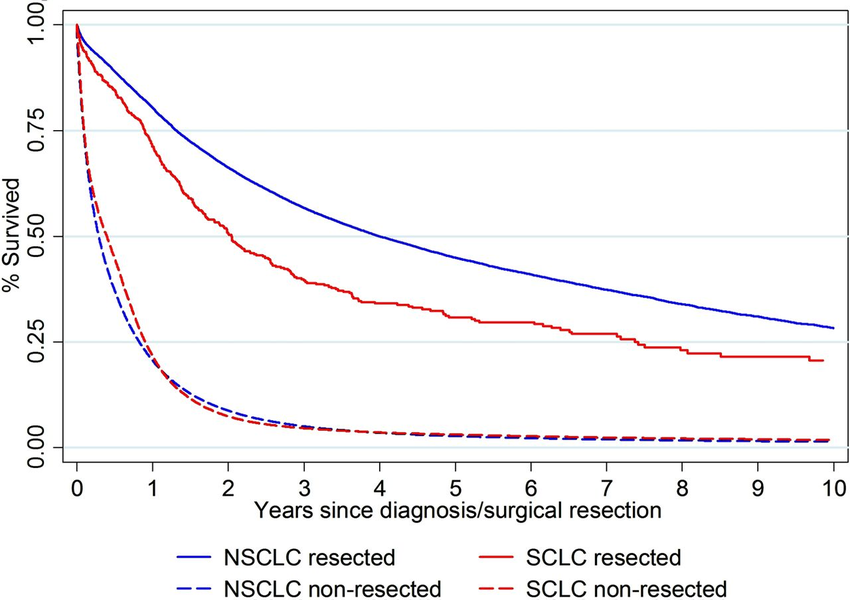
\includegraphics[width=1.00\textwidth]{../assets/05-prognosis/histological-type-survival.png}

    \small\textit{Kaplan–Meier survival analysis of resected and unresected patients with non-small 
    cell lung cancer (NSCLC) and small cell lung cancer (SCLC). \cite{article}}
\end{center}
\vspace{1em}

\begin{itemize}
    \item \textbf{Performance Status:} A measure of a patient’s general well-being and ability to 
    perform daily activities. Patients with good performance status tend to tolerate aggressive 
    treatments better and have improved survival outcomes \cite{basch2016symptoms}.

    \item \textbf{Genetic and Molecular Markers:} Certain genetic mutations, such as EGFR, ALK, or 
    KRAS, can influence prognosis and guide the use of targeted therapies. For example, patients 
    with EGFR mutations may benefit significantly from tyrosine kinase inhibitors, improving 
    survival outcomes \cite{molecular2023}.

    \item \textbf{Comorbidities:} The presence of other chronic conditions such as chronic 
    obstructive pulmonary disease (COPD), cardiovascular disease, or diabetes can affect treatment 
    options and survival \cite{copdlungcancer}.
\end{itemize}

\begin{itemize}
    \item \textbf{Smoking Status:} Non-smokers or those who have quit smoking tend to have better 
    clinical outcomes compared to current smokers. Continued tobacco exposure during treatment can 
    reduce the efficacy of therapies and worsen prognosis \cite{gilbert2020smoking}.
\end{itemize}

\vspace{1em}
\begin{center}
    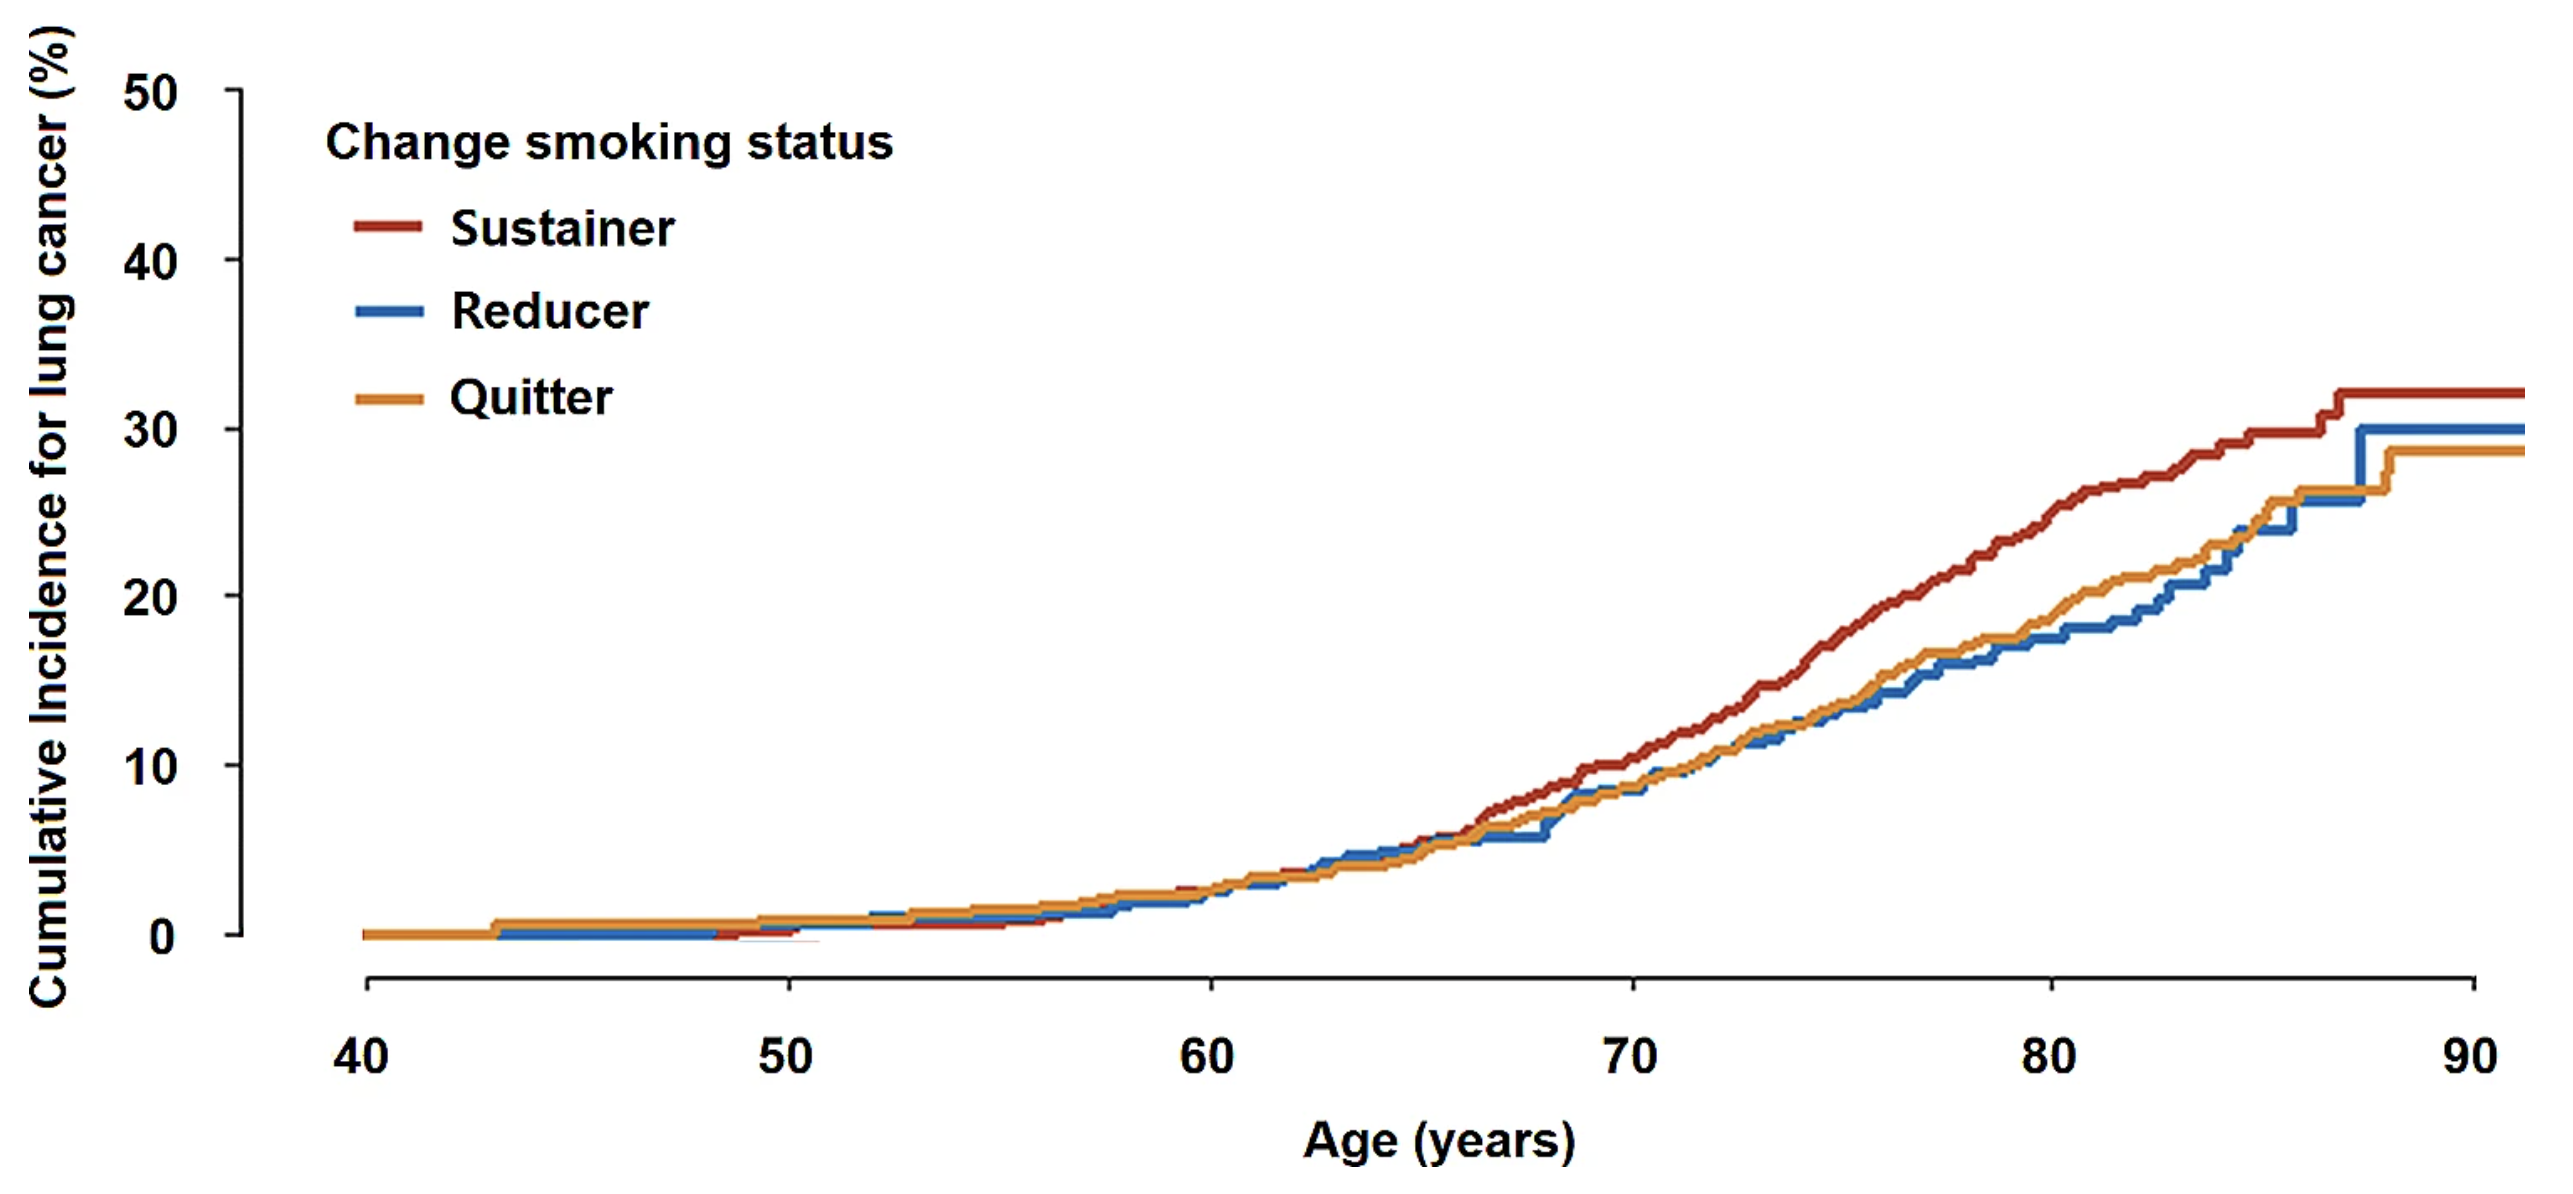
\includegraphics[width=1.00\textwidth]{../assets/05-prognosis/smoking-clinical-outcomes.png}

    \small\textit{Impact of smoking reduction on lung cancer risk in patients with COPD. 
    \cite{shin2024impact}}
\end{center}
\vspace{1em}

Understanding these prognostic indicators allows healthcare providers to make informed decisions 
regarding treatment intensity, follow-up strategies, and patient counseling. As precision medicine 
advances, integrating clinical, molecular, and lifestyle data will continue to refine prognostic 
models for lung cancer patients.

